% !TEX root = ../thesis.tex
% behavior at simple misalignments
% @author Tobias Wulf
%

\section{Verhalten bei einfachen Fehllagen}\label{sec:exp5}

\textbf{Zweck:} Das Experiment ist als Stichprobenexperiment für räumliche Fehllagen des Sensors und Verkippungen des Magneten zu betrachten und soll erste Einschätzungen des Verhalten bei einfachen Fehllagen liefern. Für eine vollständige Charakterisierung des Sensormodells muss in einem abgesteckten räumlichen Bereich jede Position mit jeder möglichen Verkippung angefahren werden. Dieses würde allerdings den Rahmen dieser Arbeit weit überschreiten und muss gesondert in nachfolgenden Arbeiten durchgeführt werden. Das Experiment ist wird mit $N_{Ref} = 17$ Referenzwinkeln für das Regressionsmodell nach mit euklidischer Abstandsfunktion nach \autoref{eq:de2innorm} und resultierender Kovarianzfunktion nach \autoref{eq:kfun} durchgeführt. Das Modell wird als mittwertfreier Kernel betrieben.

\textbf{Durchführung:} Zum Beginn des Experiments werden Drift Parameter für die räumlichen Verschiebungen des Sensors und der Verkippung des Magnet gesetzt. Basierend darauf werden im Anschluss alle notwendigen Datensätze automatisch generiert und indiziert. Es wird eine Referenzposition bei $(0;0;7,5)^T$ mm unter dem Magneten und $\SI{0}{\degree}$ Magnetverkippung festgelegt. Auf dieser Position wird ein Referenzmodell einmalig trainiert. Beginnend mit der Verschiebung in $X$ wird jeder Drift sequentiell hintereinander ausgeführt. Es folgen Drift in $Y$ und $Z$, sowie abschließend die Verkippung des Magneten. In $X$ $Y$ und $Z$ wird der Sensor jeweils um $\pm 3$ mm in $0,25$ mm Schritten relativ zur Referenzposition versetzt. Für den Drift in $Z$ deckt das ungefähr den Bereich von Sättigung bis Kennfeldmittelpunkt des TMR-Sensor-Kennfeldes ab, siehe \autoref{ch:tdk-datensatz}. Die Verkippung des Magneten wird von $\SI{0}{\degree}$ bis $\SI{12}{\degree}$ in $\SI{0,5}{\degree}$ Schritten vorgenommen. Bei jeder Driftposition wird eine volle Rotation mit $720$ Simulationswinkel bei einer Auflösung von $\SI{0,5}{\degree}$ durchgeführt. Es werden absolute Winkelfehler des Referenzmodells für den mittleren und maximalen Fehler auf die volle Rotation ausgewertet. Zusätzlich zum Referenzmodell wird ein zweites Modell mit gleich Konfiguration initialisiert. Dieses wird bei jedem Drift auf die aktuelle Position trainiert, was ein erneutes Trainieren des Referenzmodells simulieren soll. Für das zweite Modell werden ebenfalls mittlerer und maximaler Winkelfehler erfasst, sowie die Modellparameter $\sigma_f^2$, $\sigma_l$ und das Rauschniveau $\sigma_n^2$. Im Vergleich zu \autoref{sec:exp4} sind hier die Parametergrenzen geweitet und die Durchlaufzahl der Optimierung erhöht, um den Algorithmen genügend Reserve zur Verfügung zu stellen und das Verletzen von Parametergrenzen zu verhindern. Der Simulation nachfolgend werden Best- und Worst-Case Positionen des Experiments separat simuliert und im detaillierter Dargestellt.


\clearpage


\textbf{Erzeugte Datensätze:} Jeweils 100 Trainings- und Testdatensätze mit korrespondierenden Positionen des Sensors und Verkippungswinkel des Magneten. Die Datensätze werden zum Beginn des Experiments entsprechend der Driftvorgaben prozessiert, indiziert und zur Driftausführung geladen.

\textbf{Matlab-Skript:} compareMissAlign.m und demoGPRModule.m, siehe \autoref{mcode:comparemissalign} und \autoref{mcode:demogprmodule}.

\textbf{Abweichende Parameter von \autoref{tab:sim-params-exp}:}

\begin{itemize}
	\item TrainingsOptions: nAngles: 17
	\item TrainingsOptions/ TestOptions: xPos/ yPos: $-3:0,25:3$
	\item TrainingsOptions/ TestOptions: zPos: $4,5:0,25:10,5$
	\item TrainingsOptions/ TestOptions: tilt: $0:0,5:12$
	\item GRPOptions: kernel : 'QFCAPX'
	\item $\sigma_f^2$-Bounds: $(0.1,100)$
	\item $\sigma_l$-Bounds: $(1,100)$
	\item $\sigma_n^2$-Bounds: $(10^{-7},10^{-3})$
	\item GPROptions: mean: 'zero'
	\item OptimRuns 30
\end{itemize}

\textbf{Ergebnisse:} Die Ergebnisse der Simulation sind grafisch ausgewertet. In \autoref{fig:drift-model-errors} sind die Winkelfehler in Bezug auf Verschiebung des Sensors und Verkippung des Magneten erfasst.
\autoref{fig:drift-horizontal-model-parms} und \autoref{fig:drift-vertical-model-parms} zeigen, die während des Experiments festgehalten Modellparameter bei horizontalen und vertikalen Drift sowie Verkippung. In \autoref{fig:z-pos-comp-45-105-rotation} ist der Best-Case bei Drift in $z = 0,45$ mm und der Worst-Case bei Drift in $z = 10,5$ mm gesondert nebeneinander dargestellt.


\clearpage


\textbf{Beobachtungen:} Der Drift des Referenzmodell zeigt in \autoref{fig:drift-model-errors}, dass das Sensormodell sensibler auf vertikalen als auf horizontalen Versatz reagiert. Für die horizontale Verschiebung in $X$ und $Y$ zeichnet sich ein Pufferbereich von $\pm 0,5$ mm ab. Eine entsprechende Reaktion auf vertikalen Versatz in $Z$ zeigt schon bei $\pm 0,25$ mm vor. Die Winkelfehler nehmen dann exponentiell bei Vergrößerung des Versatzes zu. Im $Z$-Drift von $6,25$ mm bis $4,5$ mm stagniert der mittlere Winkelfehler. Im $X$-Drift ab $\pm 2,75$ mm kommt es zu Intervallüberschreitungen in der $\textrm{atan2}$-Funktion bei der Winkelrückrechnung, zu sehen am sprunghaften Anstieg des maximalen Winkelfehlers auf ca. $\SI{360}{\degree}$. Das trifft ebenfalls für den maximalen Winkelfehler im $Z$-Drift zu, allerdings für annähernd den ganzen Versatz in beiden Richtungen. Verkippungen des Magneten zeigen auf das Referenzmodell kaum bis keinen Einfluss.
\newline
Für das zweite Modell, dass auf jeder Position trainiert wird, zeigt sich ein symmetrisches Verhalten für Versatz in $X$- und $Y$-Richtung. Der Winkel Fehler singt bei zunehmenden Versatz und nimmt ab $\pm 3$ mm wieder leicht zu. Beim verschieben in $Z$-Richtung singt der Fehler exponentiell bei Verringerung des Abstandes zum Magneten und nimmt in gleichermaßen bei Vergrößerung des Abstandes zu. Verkippungen des Magneten zeigen hier ebenso keinen Effekt. Im Gegenteil ab $\SI{5}{\degree}$ nimmt der Winkelfehler sogar geringfügig ab.
\newline
Betrachtet man die Modellparameter für horizontale Drifts in $X$ und $Y$ mit Trainieren an jeder Versatzposition in \autoref{fig:drift-horizontal-model-parms}, zeigt sich wieder das symmetrische Verhalten aus \autoref{fig:drift-model-errors}. Zudem zeigen abfallende Parameterkurven bei zunehmenden Versatz, dass die Modellkomplexität in Bezug auf die Daten abnimmt. Für das Regression Modell sind die Trainingsdaten weniger verrauscht bei Versatz, es kann diese dort nominell besser unterscheiden. Die Parametergrenzen aus der Anpassung \autoref{sec:exp4} sind bis $\pm 2$ mm in jede Versatzrichtung größtenteils eingehalten worden. Es sind neue Grenzen in Bezug auf horizontalen Versatz (rot durchgezogen) vorgeschlagen.
\newline
Bei Drift in $Z$, siehe \autoref{fig:drift-vertical-model-parms}, zeigt das Modell im Versatzbereich von $4,5$ mm bis $6,5$ mm ein relativ stabiles Verhalten in Bezug auf die Skalierungsparameter. Ab $\SI{6,5}{\milli\metre}$ Schwankt die Skalierung der Kovarianzfunktion bei starker Zunahme des Rauschniveaus. Die Darstellung der Daten in Bezug auf das Regressionsmodell verschlechtert sich mit zunehmenden Abstand. Auf Verkippung reagiert das Modell relativ stabil. Ab $\SI{5}{\degree}$ Verkippung verringert sich die Modellkomplexität sprunghaft und bleibt dann weithin stabil. Das Rauschniveau nimmt über den gesamten Verkippungsdrift stetig ab. Die Parametergrenzen aus der Anpassung \autoref{sec:exp4} sind mit einigen Ausreißern eingehalten worden. Es sind neue Grenzen in Bezug auf vertikalen Versatz und Verkippung (rot gestrichelt) vorgeschlagen.


\clearpage


\autoref{fig:z-pos-comp-45-105-rotation} zeigt für den Best-Case aus \autoref{fig:drift-model-errors} bei Z-Drift $4,5$ mm im Vergleich zum Worst-Case bei $10,5$ mm, dass bei geringen Abstand zum Magneten die Streuung der Sensor-Pixel erhöht wird. Die Sensor-Pixel überlagern sich bei einem Abstand von $4,5$ mm in $Z$ durch die lotrechte und zentrierte Position des Sensors unterm Magneten. Bei $10,5$ mm Abstand in $Z$ ist eine Streuung nur durch einen Zoom wahrnehmbar. Auf dem Kennfeld und resultierend in polarer Darstellung der Rotation zeichnen sich für den Worst-Case ersichtliche Quantisierungsfehler ab. Die Überlagerung der Sensor-Pixel ist aufgehoben. Das Regressionsmodell schafft es nicht mehr diese auszugleichen und nähert sich daher im Winkelfehlerbild der einfachen Mittlung an.
\newline
Im Vergleich dazu ist der Winkelfehler für den Best-Case sehr gering und konstant, wobei aus einfacher Mittlung ein Winkelfehler von mehreren Grad resultieren. Die Vorhersage im Best-Case ist sehr genau und sicher mit engen und konstanten Konfidenzintervallen. Im Worst-Case zeigt sich die Instabilität in den Konfidenzintervallen mit einem Vertrauensverlust bis zu $\pm\SI{2}{\degree}$.


\clearpage
\begin{landscape}
\begin{figure}[tbph]
	\centering
	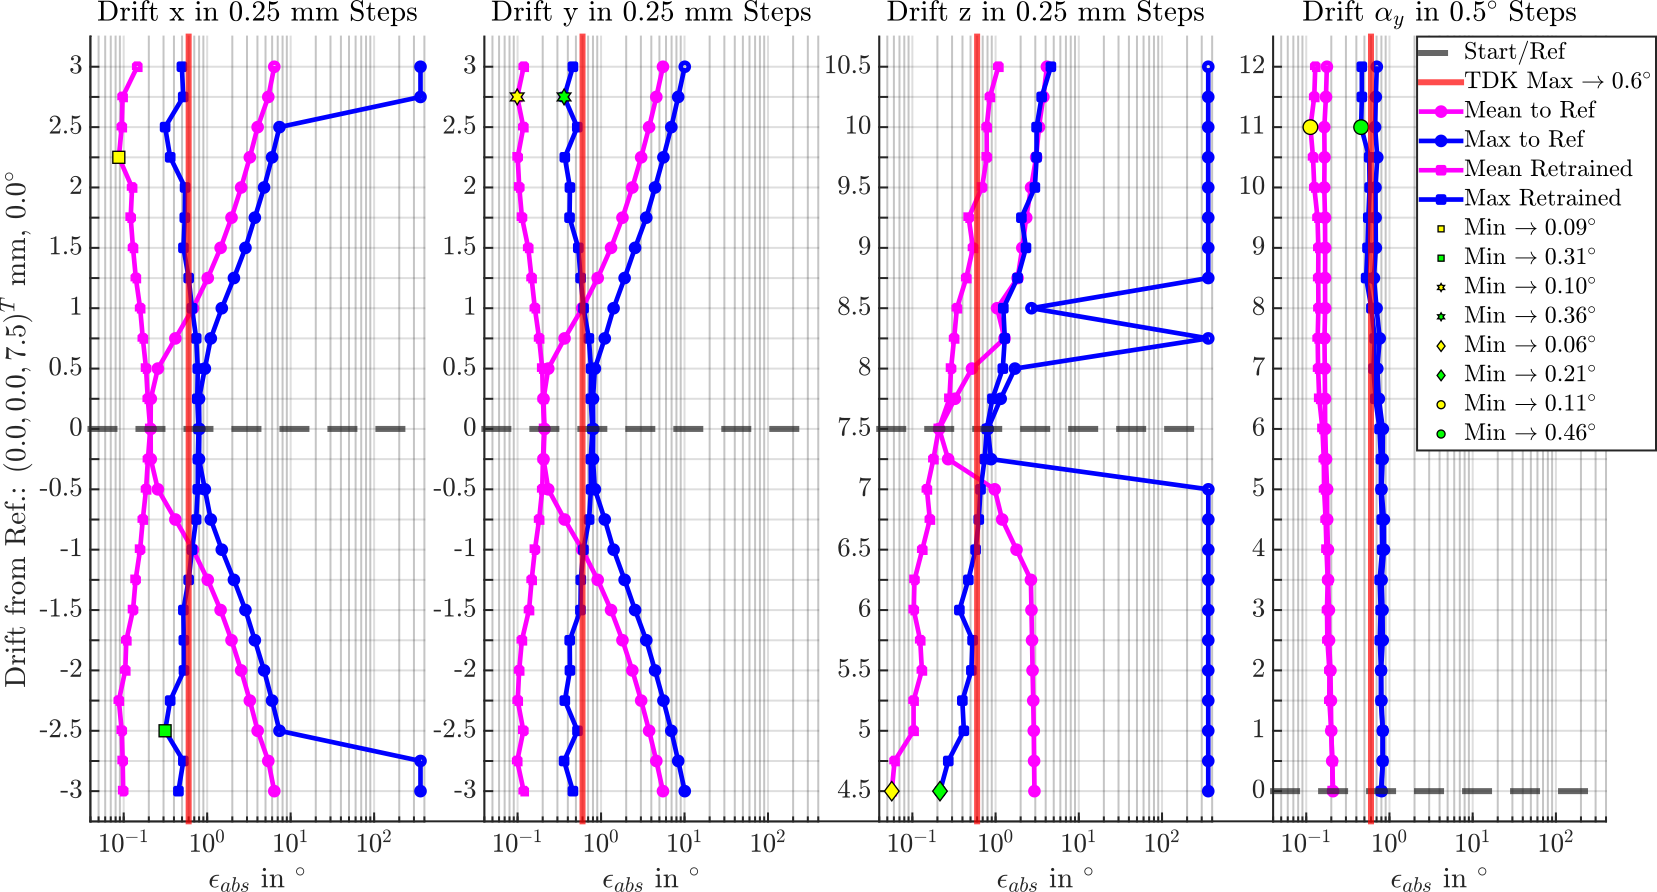
\includegraphics[width=.8\linewidth]{chapters/images/4-EuOExp/Drift-Model-Errors}
	\caption[Positionsdrift mit einfachen Versatz und Verkippung]{Positionsdrift mit einfachen Versatz und Verkippung. Simuliert sind Verschiebungen des Sensors entlang der $X-$, $Y-$ und $Z$-Achse des Koordinatensystem und Verkippung des Magneten in seiner $Y$-Achse, ausgehend von einer Referenz- bzw. Startposition bei $(0;0;7,5)^T$ mm und eine Magnetverkippung in der $Y$-Achse von $\SI{0}{\degree}$. Bei Verkippung des Magneten befindet sich der Sensor auf der Referenzposition. Es wird immer nur ein Drift z.Z. ausgeführt. Die Ausführung aller Drifte ist sequentiell. Für jeden Drift sind der mittlere und maximale absolute Winkelfehler aufgezeichnet worden. Es sind zwei Regressionsmodelle gleicher Konfiguration nach \autoref{eq:de2innorm} und \autoref{eq:kfun} als mittlerwertfreie Modelle zur Berechnung der Fehler genutzt worden. Das erste Modell ist einmalig auf der Referenzposition trainiert worden. Das zweite Modell ist bei jeder Driftposition trainiert worden (Retrained). Es ist zusätzlich der maximale Winkelfehler des TDK TMR-Sensors aufgetragen \cite{TDK2016}. Minimum der mittleren Fehler sind gelb markiert. Minimum der maximalen Fehler sind grün hervorgehoben.}
	\label{fig:drift-model-errors}
\end{figure}
\end{landscape}


\clearpage
\begin{landscape}
\begin{figure}[tbph]
	\centering
	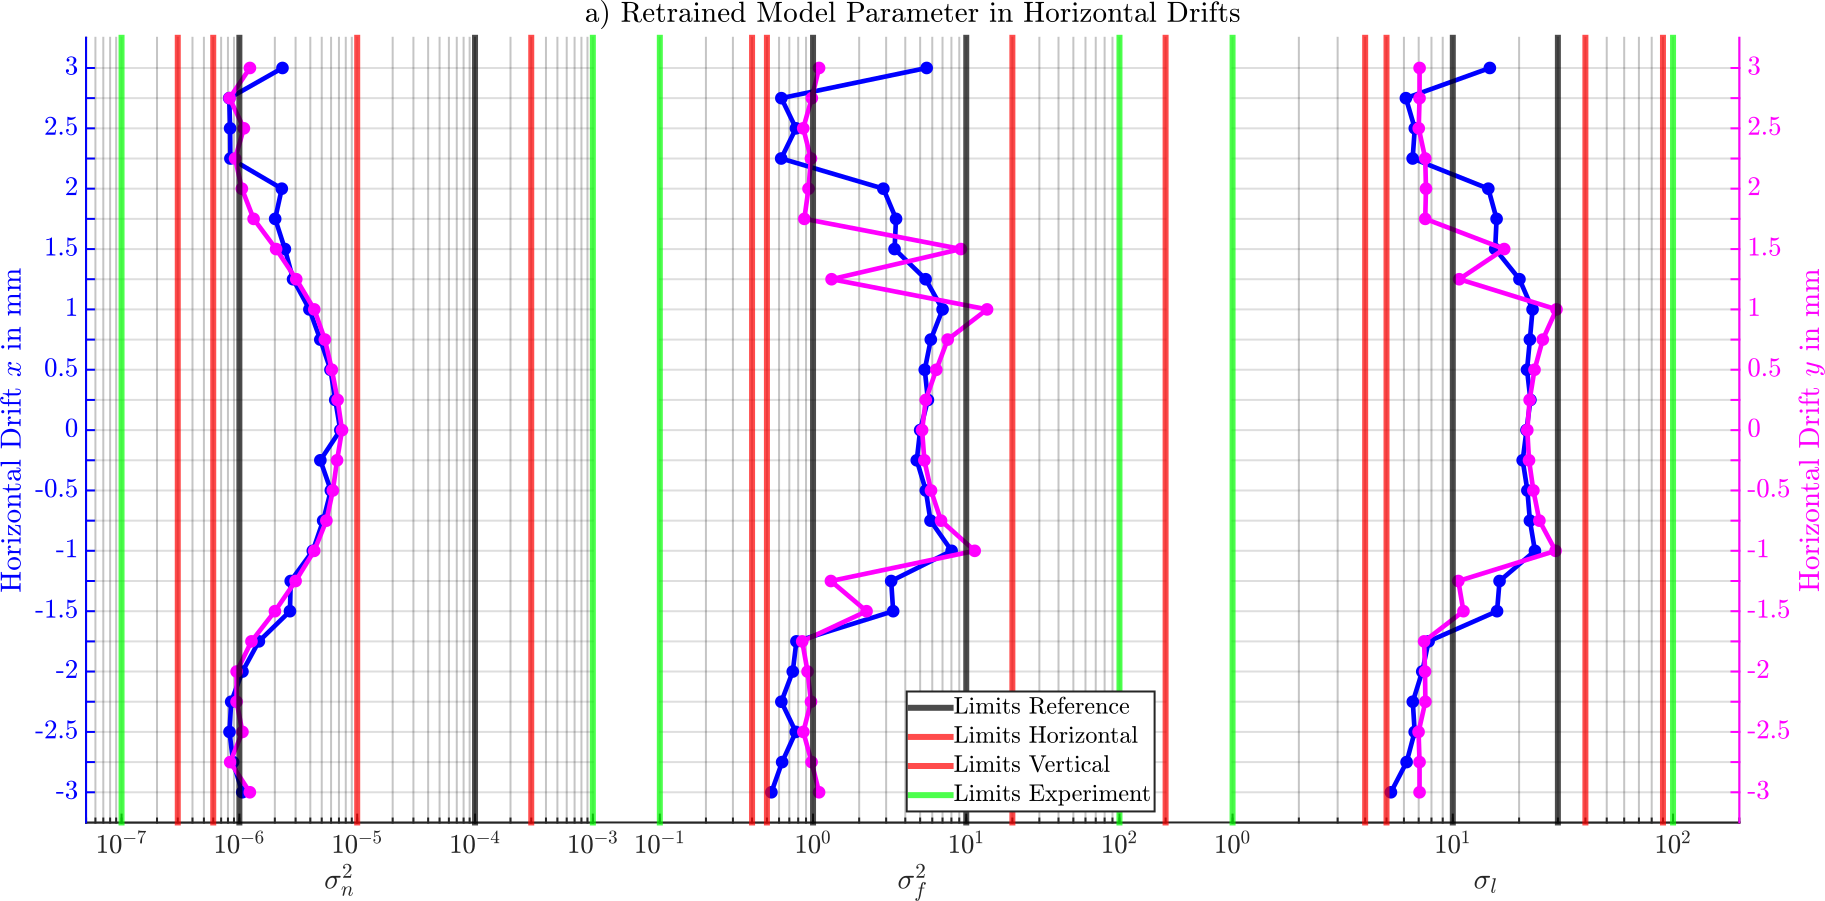
\includegraphics[width=\linewidth]{chapters/images/4-EuOExp/Drift-Horizontal-Model-Parms}
	\caption[Modellparameter bei horizontalem Drift]{Modellparameter bei horizontalen Drift. Aufgenommen sind das Rauschniveau $\sigma_n^2$ und die Höhenskalierung $\sigma_f^2$ sowie die Längenskalierung $\sigma_l$ der Kovarianzfunktion für das zweite Regressionsmodell (Retrained) aus \autoref{fig:drift-model-errors}, hier für Verschiebungen entlang der $X$-/ $Y$-Achse. Es sind Parametergrenzen als Referenz in Bezug auf Anpassungen aus \autoref{sec:exp4} aufgetragen. Zusätzlich sind die im Experiment genutzten Grenzen aufgetragen, sowie die sich hier ergebenen Grenzen aus horizontaler Verschiebung und die aus vertikaler Verschiebung bzw. Verkippung resultierenden Parametergrenzen aus \autoref{fig:drift-vertical-model-parms}.}
	\label{fig:drift-horizontal-model-parms}
\end{figure}
\end{landscape}


\clearpage
\begin{landscape}
	\begin{figure}[tbph]
		\centering
		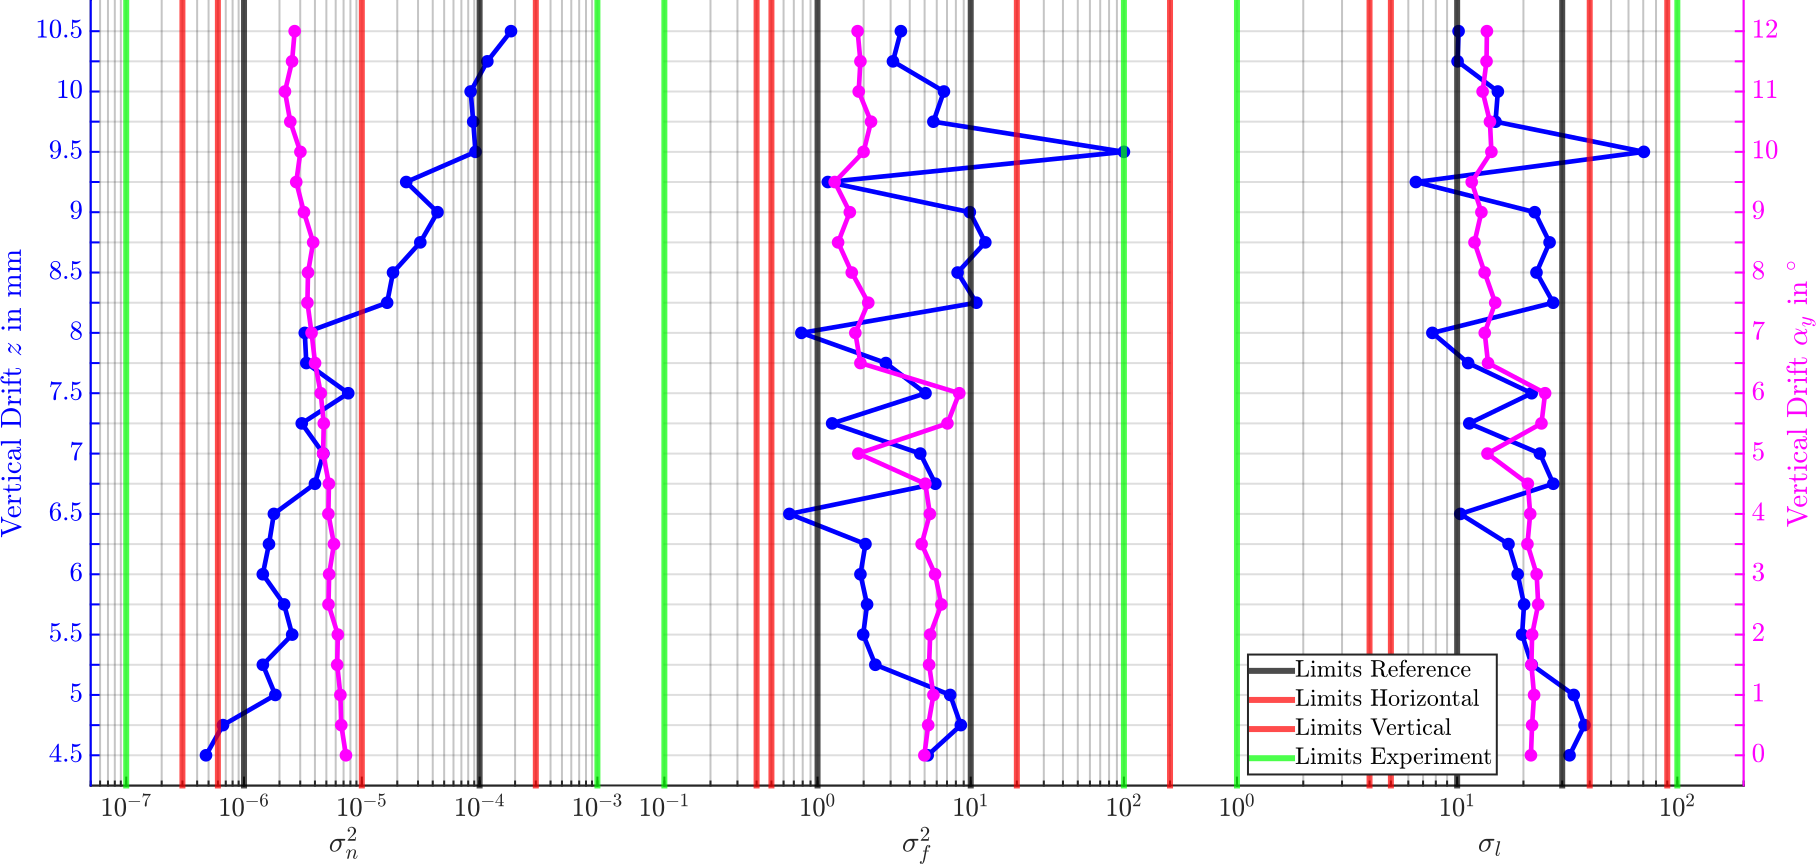
\includegraphics[width=\linewidth]{chapters/images/4-EuOExp/Drift-Vertical-Model-Parms}
		\caption[Modellparameter bei vertikalem Drift und Verkippung]{Modellparameter bei vertikalen Drift und Verkippung. Aufgenommen sind das Rauschniveau $\sigma_n^2$ und die Höhenskalierung $\sigma_f^2$ sowie die Längenskalierung $\sigma_l$ der Kovarianzfunktion für das zweite Regressionsmodell (Retrained) aus \autoref{fig:drift-model-errors}, hier für Verschiebungen entlang der $Z$-Achse und Verkippung des Magneten in der $Y$-Achse. Es sind Parametergrenzen als Referenz in Bezug auf Anpassungen aus \autoref{sec:exp4} aufgetragen. Zusätzlich sind die im Experiment genutzten Grenzen aufgetragen, sowie die sich hier ergebenen Grenzen aus vertikaler Verschiebung bzw. Verkippung und die aus horizontaler Verschiebung resultierenden Parametergrenzen aus \autoref{fig:drift-horizontal-model-parms}.}
		\label{fig:drift-vertical-model-parms}
	\end{figure}
\end{landscape}


\clearpage
\begin{figure}[tbph]
	\centering
	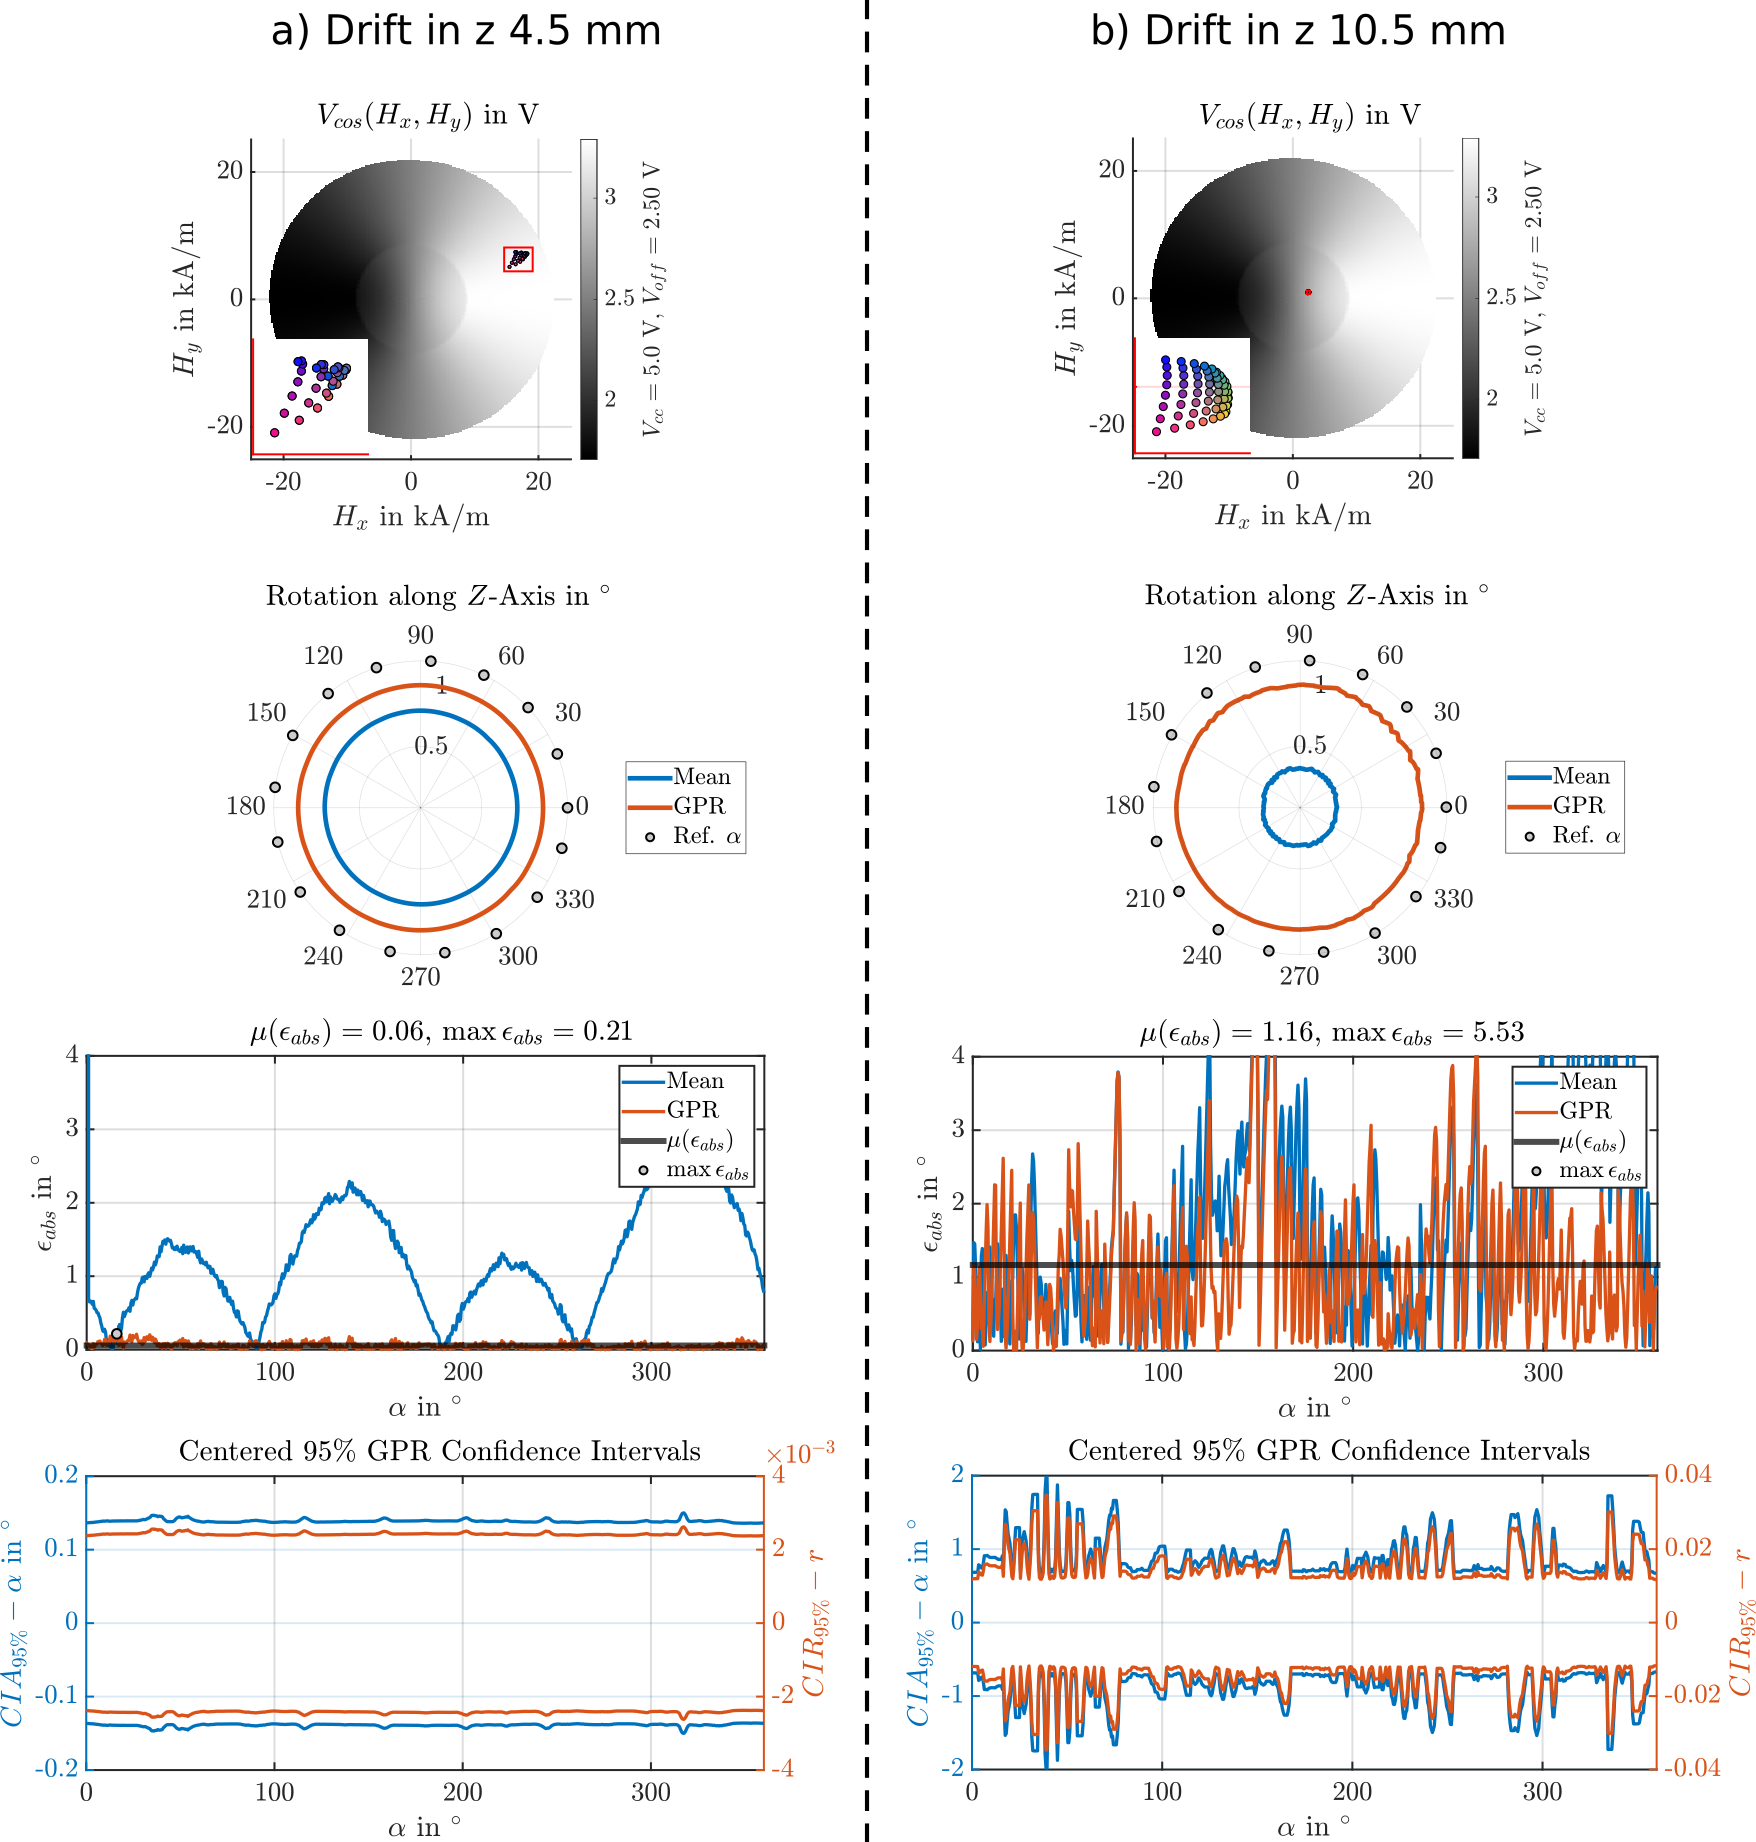
\includegraphics[width=\linewidth]{chapters/images/4-EuOExp/Z-Pos-Comp-45-105-Rotation}
	\caption[Best- und Worst-Case-Beispiel bei vertikalem Drift]{Best- und Worst-Case-Beispiel für vertikalem Drift aus \autoref{fig:drift-model-errors} für das zweite Regressionsmodell (Retrained). In a) und b) bei lotrechten und zentrierten Abstand vom Magneten ohne Verkippung. In a) mit $\SI{0,45}{\milli\metre}$ und in b) mit $\SI{10,5}{\milli\metre}$ Abstand. Für beide Beispiele ist die Sensor-Pixel-Streuung bei $\SI{21,5}{\degree}$ anhand des Kennfeldes für die Cosinus-Funktion gezeigt, sowie der Rotationsverlauf um die $Z$-Achse in Polardarstellung mit einfacher Mittlung der Daten (Mean) und Ergebnis via Gauß-Prozess-Regression (GPR) inklusive der Referenzwinkel für die GPR. Anschließend ist für beide Beispiele der absolute Winkelfehler über die volle Rotation aufgetragen mit nachfolgenden $95\%$ Konfidenzintervallen für Winkelvorhersagen (CIA) und Radius (CIR). Modelltrainingsdaten basieren auf Vektoren bzw. Skalare.}
	\label{fig:z-pos-comp-45-105-rotation}
\end{figure}


\clearpage

